\chapter{Implementation}

\section{Javascript Cryptography}

\paragraph{The developer decided that the best solution for the cryptography implementation was the utilization of a pre-existing cryptography library.}

\paragraph{For this task, there were three necessary conditions that had to be met:}

\begin{itemize}
\item A clear, easily identifiable, and reputable source/owners
\item Existing, easily obtainable, and comprehensive documentation
\item Open source, easily available code analysis
\end{itemize}

\paragraph{and, slightly less important, actively maintained.}

\paragraph{Meeting the above criteria was not as simple as it would seem. There were many options that met some of the conditions, but meeting all of them was more challenging. Ultimately, however, the researcher was satisfied with the Stanford Javascript Crypto Library (SJCL), as it met all the above conditions. Additionally, it appeared to be well developed, and still actively maintained (See: \ref{fig: exampleSJCL_js}.}\cite[Website]{SJCL}

\paragraph{The usage is uncomplicated, and will work for this implementation. The library is available in a minified version, and will be packages with the add-on:}

\begin{figure}[H]
\centering
\begin{minted}[breaklines]{javascript}
var ciphertext = sjcl.encrypt("reallyHardPasswordNoOneCouldEveryGuess", "Hello World!");
var plaintext = sjcl.decrypt("reallyHardPasswordNoOneCouldEveryGuess", ciphertext);
console.log("plain text: " + plaintext);
console.log("cipher text: " + ciphertext);
console.log("plain text - again!: " + plaintext);
\end{minted}
\caption{\label{fig: exampleSJCL_js} Example of javascript SJCL}
\end{figure}

\paragraph{giving the following result (See: \ref{fig: exampleSJCL}):}

\begin{figure}[H]
\centering
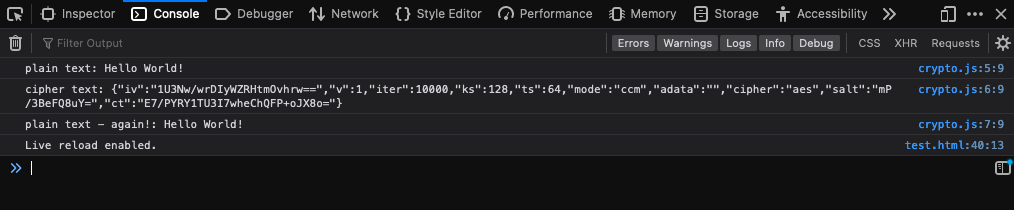
\includegraphics[width=0.9\textwidth]{exampleSJCL.png}
\caption{\label{fig: exampleSJCL} Example output to Firefox console}
\end{figure}

\paragraph{This usage will meet our needs.}

\section{WebExtensions}

\paragraph{WebExtensions are web technologies built with the tools that are natural to any web developer: HTML, CSS, and Javascript. Each extension must have a \emph{manifest.json} file, which essentially holds all the vital information like the author of the software, permissions required to use the add-on, the software version, and so on.} \cite[Webpage]{WebEx}

\paragraph{Starting with the release of Thunderbird version 68 (August 2019), Thunderbird moved to only support WebExtensions for add-ons and themes development, with all previous versions no longer working. Even the long standing Enigmail cryptography add-on that the author used for years, no longer functioned.}

\paragraph{Here is an image from Mozilla's Thunderbird Add-on Webpage that gives a quick glance of how the extensions might look like (See: \ref{fig: webEx}.} \cite[Webpage]{WebEx}

\begin{figure}[H]
\centering
\includegraphics[width=0.9\textwidth]{webEx.png}
\caption{\label{fig: webEx} WebExtension overview}
\end{figure}


\section{Implementation Details}

\subsection{Developer Tools}

\paragraph{For this project, the developer used a Test Driven Development model to go step-by-step through each implemented item. This allows for immediate checking if something works or not, and enhancement of the code in an incremental way. Most every step will be sent to the console.log, to verify success or failure. The first invaluable tool was Tunderbird's mail client Developer Toolkit, which shows a great deal of information, and includes the console. It was an excellent tool which helped with debugging, and seeing what was working and not working through each step (See: \ref{fig: devToolkit}). The developer had it open at all times. Note: Not incidentally, it looks like a typical web browsers developer toolkit, since Thunderbird's core is based on Web Extension technology.}


\begin{figure}[H]
\centering
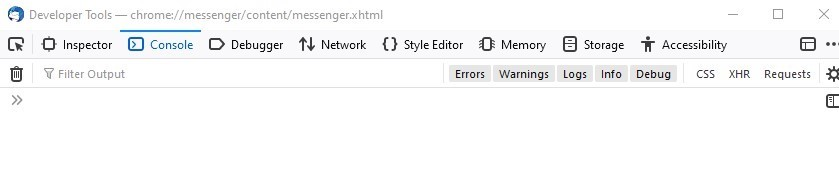
\includegraphics[width=0.9\textwidth]{developerToolKit.jpg}
\caption{\label{fig: devToolkit} Developer Toolkit}
\end{figure}

\paragraph{The second valuable tool was the communication channel Element. It an excellent channel to ask questions to other Thunderbird developers. It was where I found answers to most issues that I had (See: \ref{fig: helpScreeny}).}\footnote{https://element.io/}

\begin{figure}[H]
\centering
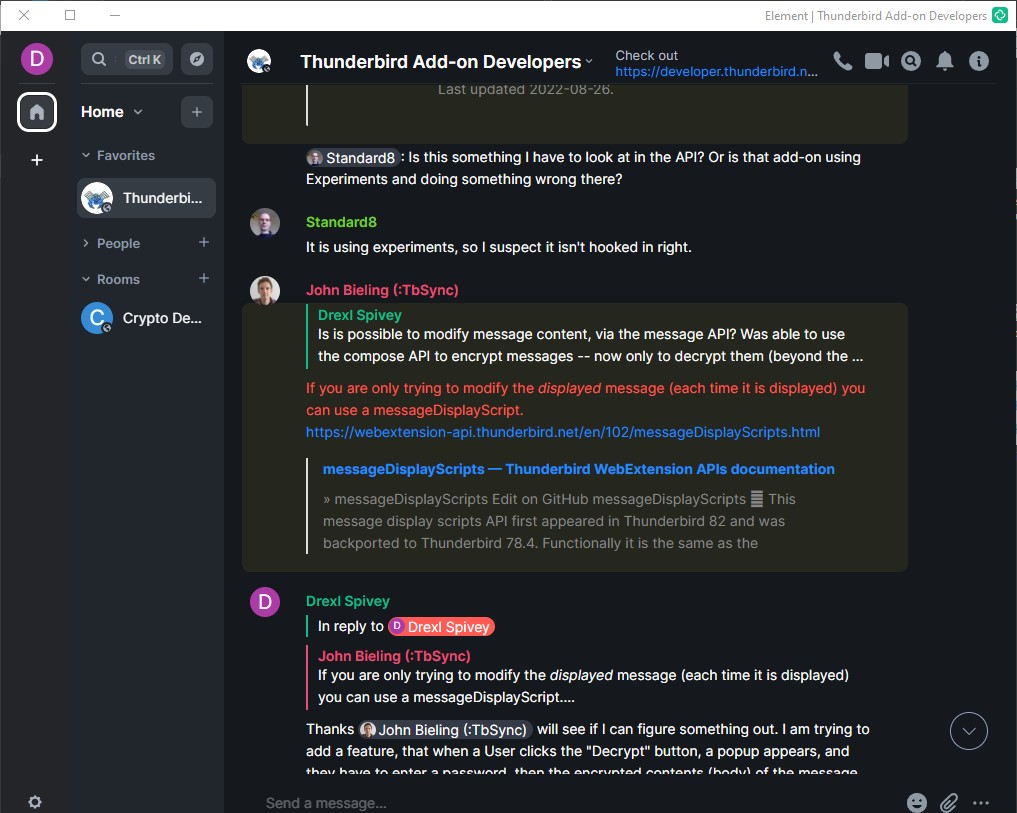
\includegraphics[width=0.9\textwidth]{helpScreeny.jpg}
\caption{\label{fig: helpScreeny} Developer uses Element (Drexl Spivey)}
\end{figure}

\paragraph{As mentioned in the acknowledgements, John Bieling was always able to point me in the right direction, within a reasonably short period of time. So, this type of quick responses were paramount to getting the author back on track.}

\paragraph{The third valuable resource gained during the development process was a Github repository that had many sample extensions. The examples that provided the most help are listed below:}\cite[Website]{Bieling}

\begin{enumerate}
\item awaitPopup
\item myComposeBody
\item messageDisplayScript
\end{enumerate}


\subsection{Creating a compose window encryption button}

\paragraph{First, we'll create a button that will appear in the "Compose Window," the window that appears when you start to write an email.}

\paragraph{Before add-on implementation: (See: \ref{fig: noButton})}

%add image here
%add Image
\begin{figure}[H]
    \centering
    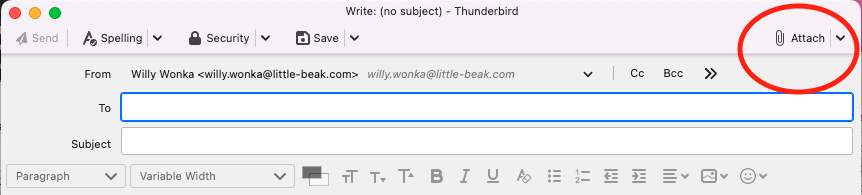
\includegraphics[width=0.9\textwidth]{ComposeWindow_No_Button.png}
    \caption{\label{fig: noButton} Normal compose window}
\end{figure}

\paragraph{with add-on button implemented (See: \ref{fig: withButton}).}

%add Image
\begin{figure}[H]
    \centering
    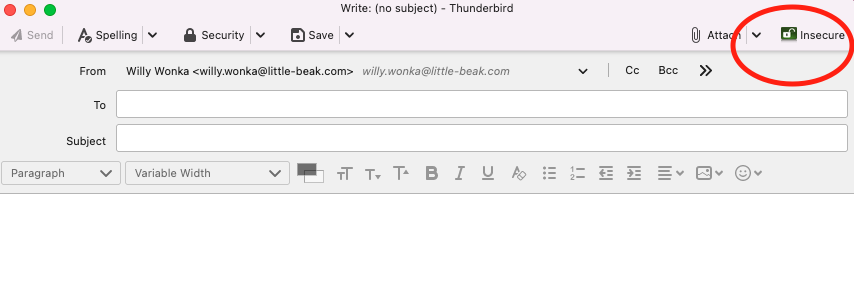
\includegraphics[width=0.9\textwidth]{ComposeWindowButtonInsecure.png}
    \caption{\label{fig: withButton} Button added to the compose window.}
\end{figure}

\paragraph{And, here is the manifest.json file that was created for this button. Most of the references in the manifest.json file are self-explanatory. One thing to note about the manifest file is the version number. It has to be set to 2. The rest is composed of information about the add-on, location of images used, and the permissions required for the add-on to function, which is not insignificant. Different permissions are required to access different areas of the user interface, e.g. the compose window, browser window, messages, modifyMessages, etc. (See reference figure: \ref{fig: basic_manifest.json}).}

%add code here
\begin{figure}[H]
\centering
\begin{minted}[breaklines]{javascript}
{
    "manifest_version": 2,
    "name": "Crypto add-on",
    "description": "A password AES cryptographic addon",
    "version": "1.5",
    "author": "Esteban Licea",
    "applications": {
        "gecko": {
            "id": "esteban@little-beak.com",
            "strict_min_version": "78.0"
        }
    },
    "compose_action": {
        "default_title": "Insecure",
        "default_icon": "images/unlocked_64px.png"
    },
    "permissions": [
        "menus"
    ]
}
\end{minted}
\caption{\label{fig: basic_manifest.json} Basic manifest.json file}
\end{figure}

\subsection{Prompt for password}

\paragraph{Managing the password was an early obstacle encountered. Namely, the developer was put on notice that he simply could not just use straight Javascript to get the desired results, but instead had to work within the context of Mozilla's API. So, this was an initial challenge.}


\paragraph{I wanted to highlight the process one time, just so it's clear. This was the process throughout. First, if necessary, the manifest.json file has to be updated. Then, the web extension files (HTML, CSS, and Javascript) should be kept orderly. But, additionally, Mozilla web extension API rules needed to be followed.}

\paragraph{Step one: updated the manifest.json file. The developer needed to add the \emph{compose\_action} so that the button would be added on the compose window.}


%add code here
\begin{figure}[H]
\centering
\begin{minted}[breaklines]{javascript}
{
    "compose_action": {
        "default_popup": "passwordPrompt/passwordPrompt.html",
        "default_title": "Insecure",
        "default_icon": "images/unlocked_64px.png"
    },
}
\end{minted}
\caption{\label{fig: addPwToManifest} Add a Password Prompt to manifest file}
\end{figure}


\paragraph{But, in the code, several files needed to be created, in addition to the pop up folder. A \emph{background.js} file needed to be created. The background.js file acts, as the name suggests in the background. It is loaded when the add-on is loaded, and it is running, or shall I say, "listening" for events. The code will be available on github, but I will explain the basic process.}

\paragraph{The background.js listeners are just waiting for the encrypt button to be clicked. This activates the pop up window, which will launch the popup.html file. (See: \ref{fig: withButton}}

%add Image
\begin{figure}[H]
    \centering
    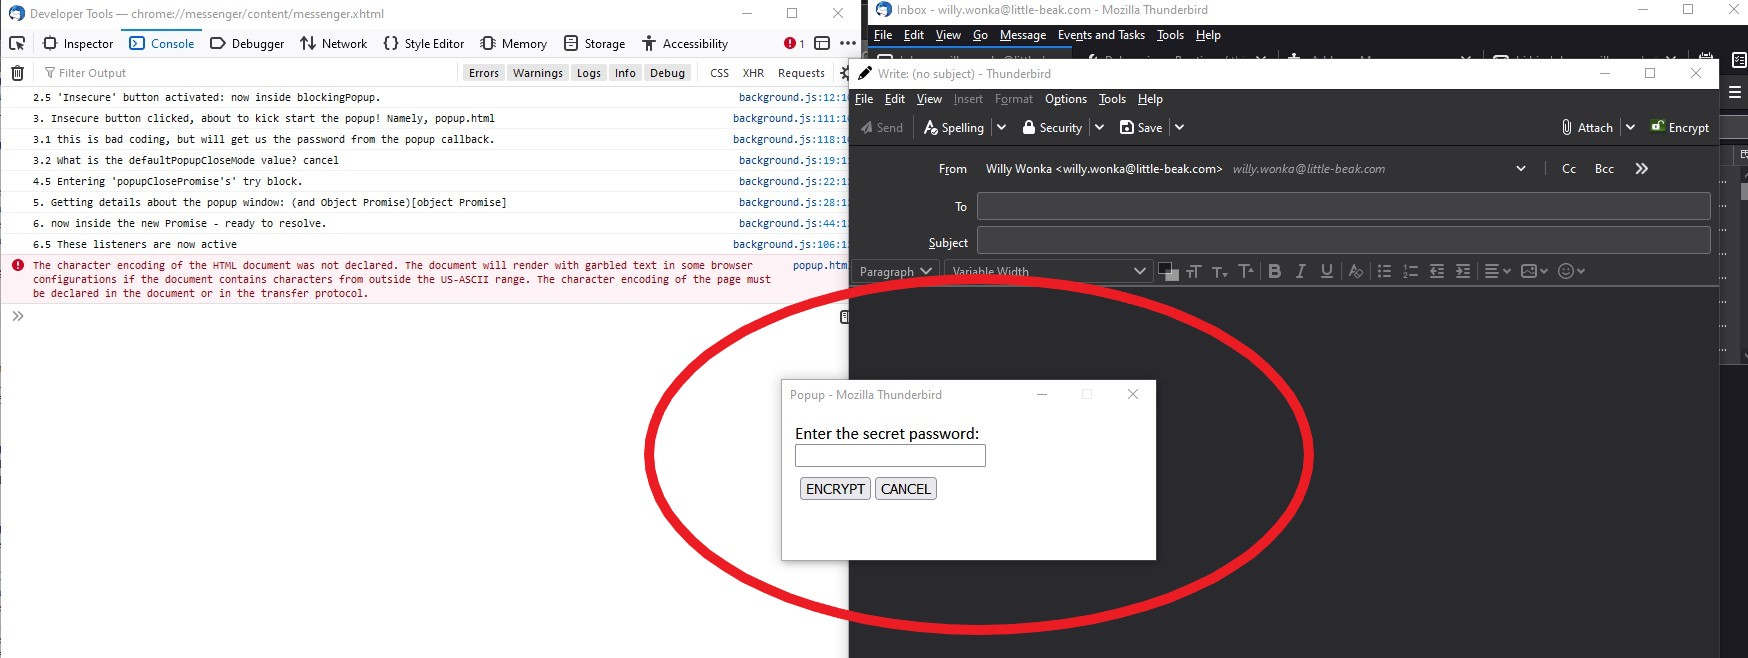
\includegraphics[width=0.9\textwidth]{passwordPopup.jpg}
    \caption{\label{fig: withButton} Pop up Window with Developer Toolkit}
\end{figure}

\paragraph{The reader can notice how I used the Developer Toolkit, with console.log used literally throughout the development process.}

\subsection{Encrypt the message}
\paragraph{The challenge with the password was not simply collecting it. But, instead, it was passing the variable from the popup.html and its accompanying popup.js to the background.js. The way the API works, it wasn't as straight forward as the developer originally thought. The password had to be sent as a message, to listeners in the background.js.}

\paragraph{Fortunately, there were some examples that were reasonably close on Mr. Bieling's github sample-extensions repo that gave me some ideas of how it could work.}

\paragraph{The encryption was a three part process:} 

\begin{itemize}
\item Get the password variable
\item Load the Stanford Javascript Cryptography Library
\item encrypt away! Hopefully. 
\end{itemize}

\paragraph{After we were able to move the password variable to the background.js, we could go with step two.}

\paragraph{For this step, the developer loaded the minimized version of the library, which is quite small, and still powerful. This is how it was loaded into the background.js file. (See: \ref{fig: loadSJCL})}


%add code here
\begin{figure}[H]
\centering
\begin{minted}[breaklines]{javascript}
var imported = document.createElement('script');
imported.src = 'sjcl.js';
document.head.appendChild(imported);
\end{minted}
\caption{\label{fig: loadSJCL} Loading external library into background.js}
\end{figure}

\paragraph{During development, every step was sent to the console.log (later cleaned up). There are a few different elements here to take note of. Firstly, some of the elements are part of the Mozilla API, like the details.body, messenger.compose.setComposeDetails. Apparently, the messenger is the namespace used for Thunderbird, replacing what was previously used (the browser namespace).}

\paragraph{Another interesting component is the actual execution of the encryption, by the SJCL.}\footnote{Stanford Javascript Cryptography Library}

\paragraph{It's usage is simple, it takes two arguments, one with a password, and another with the text to be encrypted.}


%add code here
\begin{figure}[H]
\centering
\begin{minted}[breaklines]{javascript}
let password = popupCloseMode;
console.log("16. Encrypting now! " + sjcl.encrypt(password, details.body));
console.log("12. Random text to encrypt is: " + details.body);
let newBody = sjcl.encrypt(password, details.body);
console.log("17. newBody is " + newBody);
messenger.compose.setComposeDetails(currentComposeTabId, { body: newBody })
\end{minted}
\caption{\label{fig: encryptionCode} Encryption code}
\end{figure}

\paragraph{The expected and natural behavior for a user is for them to write an email, then click on the "encrypt" button, like so. (See: \ref{fig: button}), and enter a password.}

%add Image
\begin{figure}[H]
    \centering
    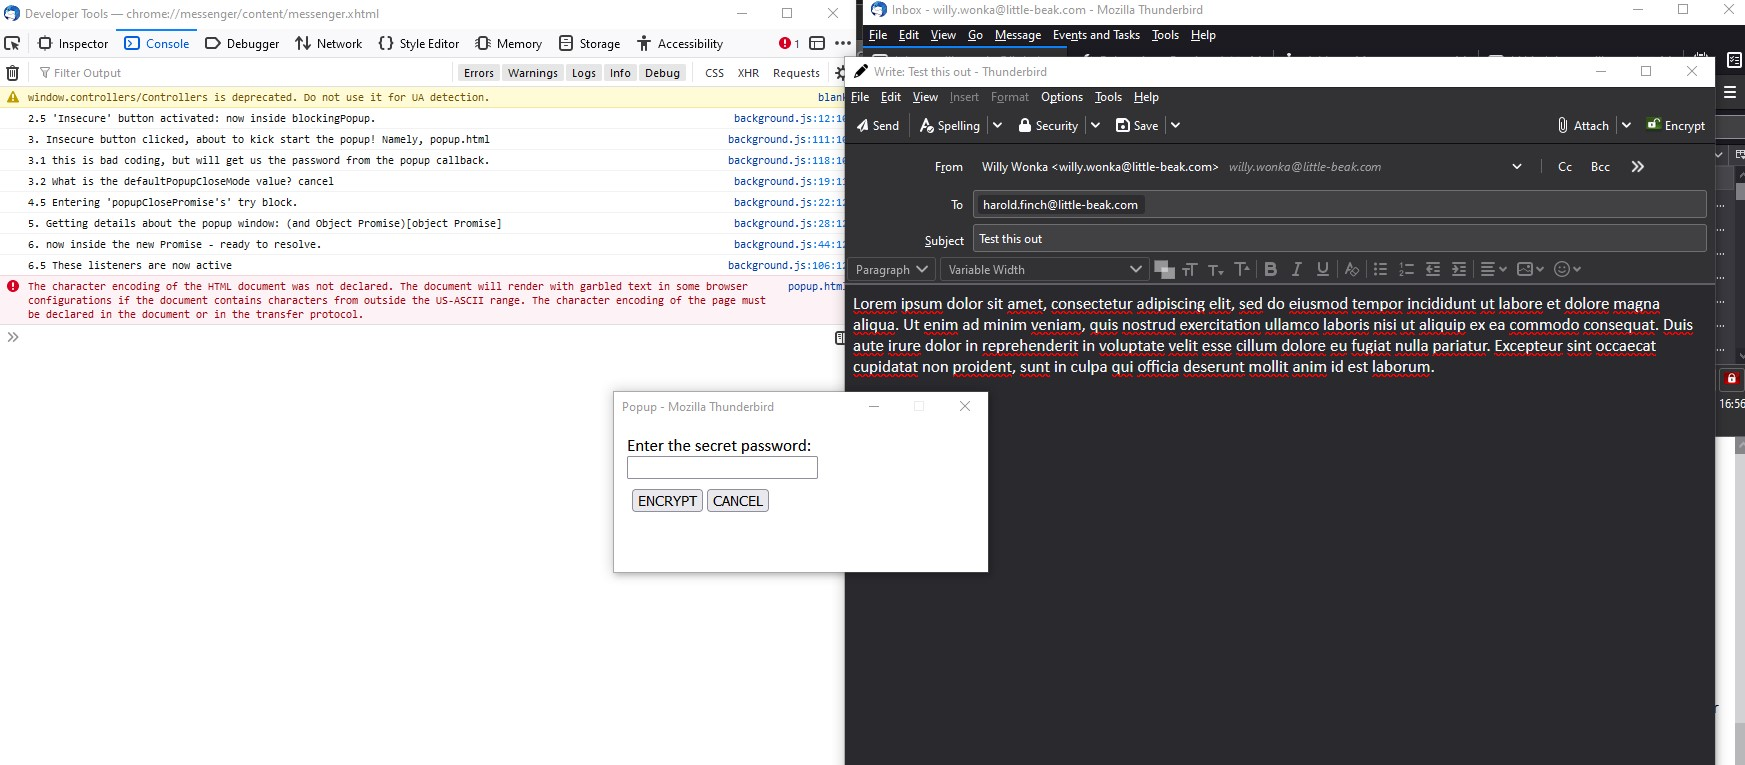
\includegraphics[width=0.9\textwidth]{step2.jpg}
    \caption{\label{fig: button} The popup window, in front of a completed email}
\end{figure}

\paragraph{After that, a password is entered, and the magic happens. (See: \ref{fig: encryptedText})}

%add Image
\begin{figure}[H]
    \centering
    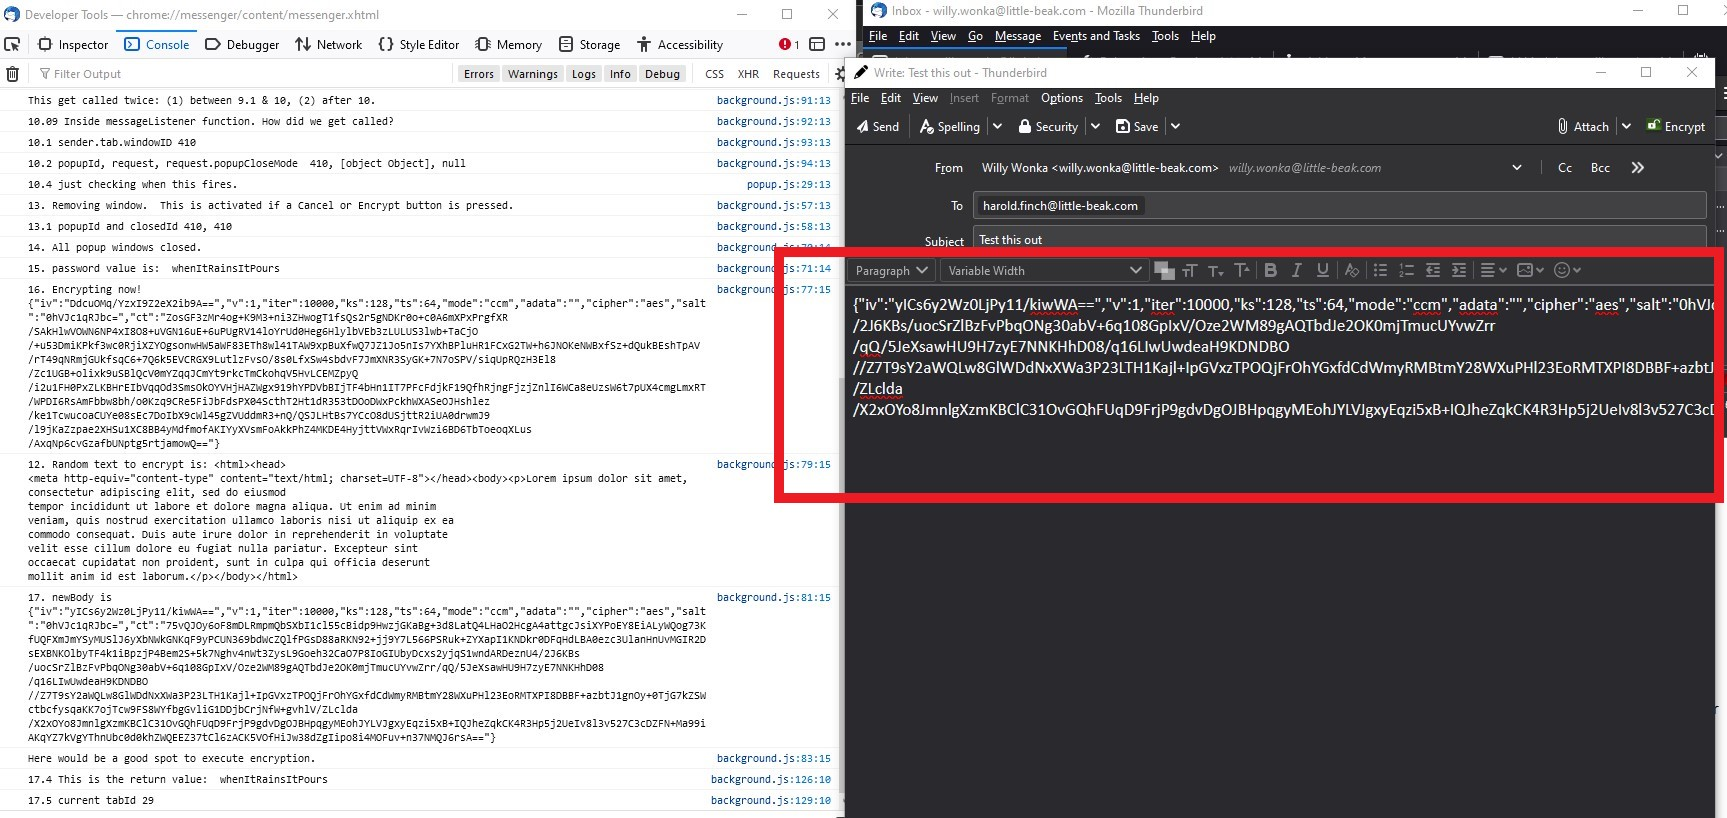
\includegraphics[width=0.9\textwidth]{step3.jpg}
    \caption{\label{fig: encryptedText} Voila! Encrypted text}
\end{figure}

\paragraph{Note: the console.log keeping track of where we are, and also verifying that the decryption also works with the same password. From here, the message can be sent as normal, or saved as a draft. There was some developmental pondering, if the encryption button should also send the message in one go, since it's not like the email is really able to be edited or read at this point, but for now left it as is, giving the user the option to add attachments or email recipients.}


\subsection{Decrypt the Message}
\paragraph{Now, sending the email to another account, we can see two very interesting elements.}

\paragraph{First, there is a "Decrypt" icon on the far right of what is known as the \emph{message\_display\_area} another UI component of the Thunderbird interface. (See: \ref{fig: decryptButton})}

%add Image
\begin{figure}[H]
    \centering
    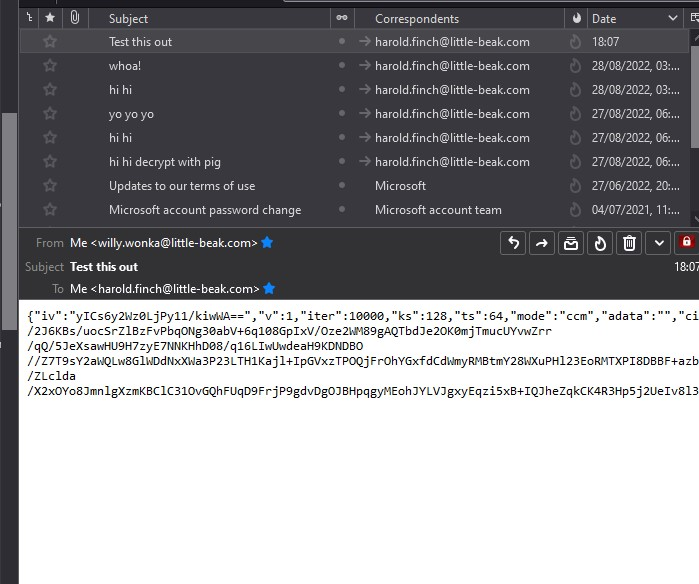
\includegraphics[width=0.9\textwidth]{step5.jpg}
    \caption{\label{fig: decryptButton} Decrypt icon}
\end{figure}


\paragraph{This is another required manifest.json addition, as well as updating the permissions section (See: \ref{fig: updateManifest} \& \ref{fig: decrypt1}).}

%add code here
\begin{figure}[H]
\centering
\begin{minted}[breaklines]{javascript}
"message_display_action": {
  "default_title": "Decrypt",
  "default_icon": "images/locked_64px.png"
},
"permissions": [
    "compose",
    "messageRead",
	"messagesModify"
]
\end{minted}
\caption{\label{fig: updateManifest} Updated manifest.json components}
\end{figure}

\paragraph{An interesting encryption component that has not been explained, is the way the encrypted message is displayed. Most of the encrypt text describes the protocols involved, like mode of operation (in this case, CCM, or \emph{Counter with Cipher Block Chaining-Message Authentication Code}), type of cipher used (AES), the version, etc. What leads the block, however, is important. The "iv" or the \emph{Initialization vector}. This is essentially used as a seeding value. And what is so interesting about it is: that even if a would be hacker was given the "iv" value, without the password they would be no closer to decrypting the message. (See \ref{fig: decrypt1})}\cite[p.170]{Schneier}

\paragraph{The following image displays the activation of the "decrypt button" which displays a similar pop-up window as was shown during the encryption pop-up, with the only difference between "ENCRYPT" or "DECRYPT," naturally.  (See \ref{fig: decrypt1})}


%add Image
\begin{figure}[H]
    \centering
    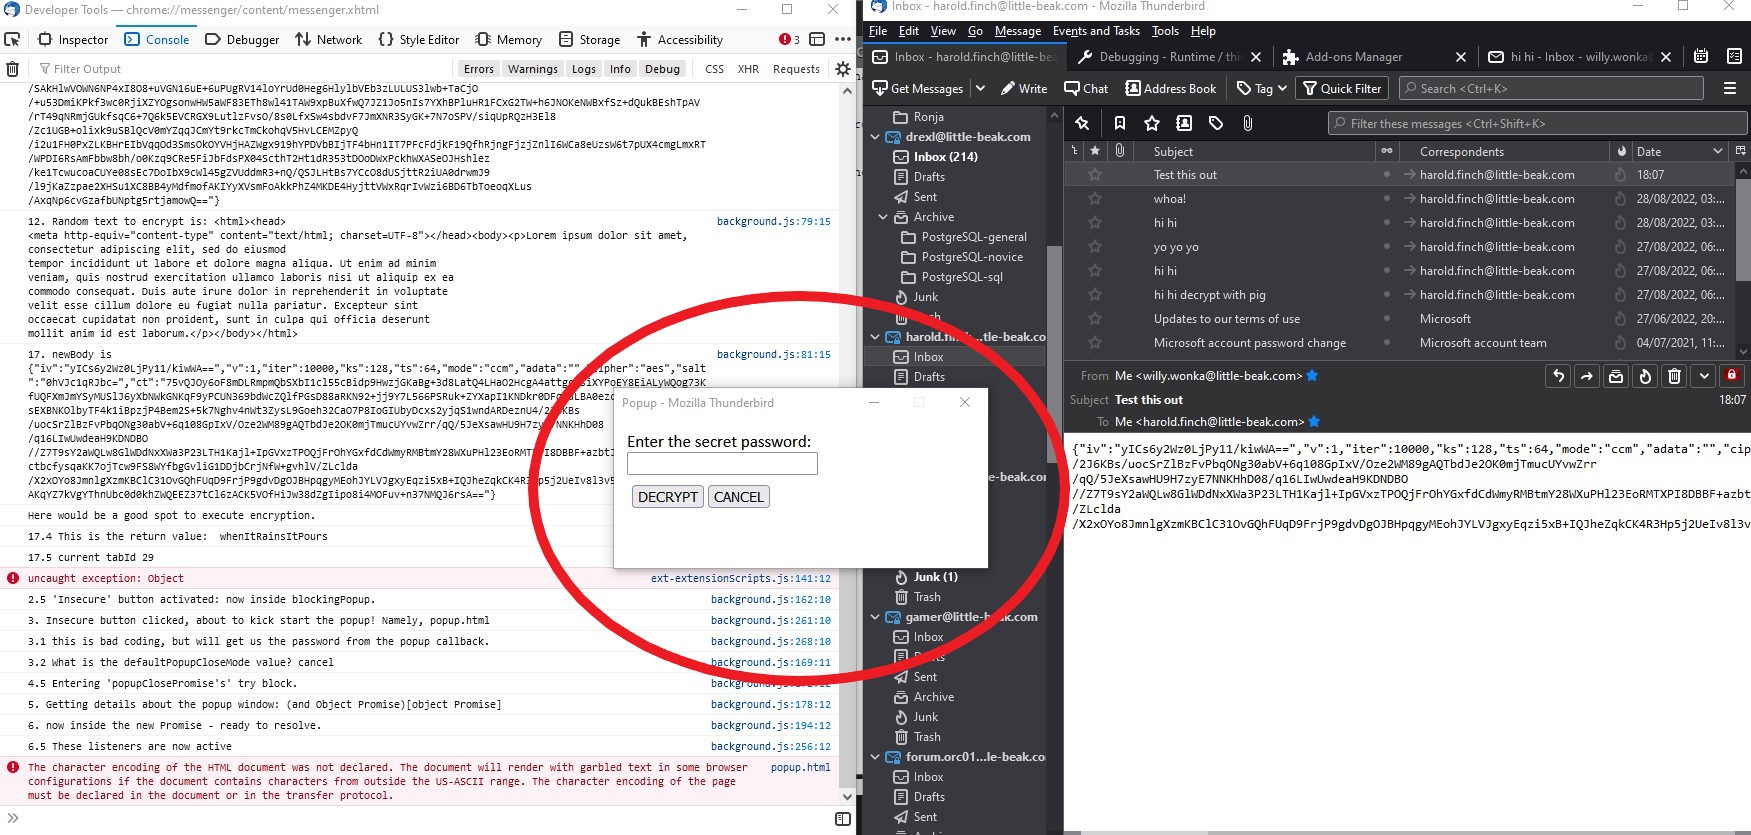
\includegraphics[width=0.9\textwidth]{step6.jpg}
    \caption{\label{fig: decrypt1} Decryption button activating pop-up}
\end{figure}

\paragraph{Finally, in the console.log, we are able to see that from the receiving end, we are able to decrypt the emailed text when the correct password is given. (See: \ref{fig: decrypt2})}


%add Image
\begin{figure}[H]
    \centering
    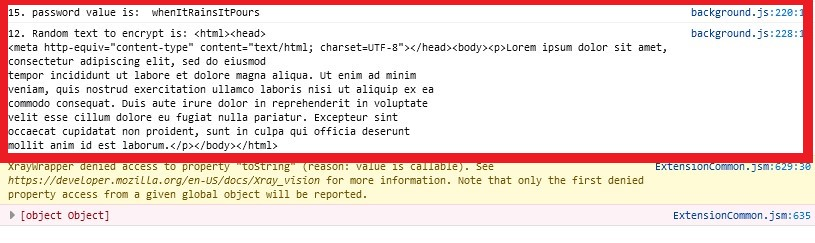
\includegraphics[width=0.9\textwidth]{step7.jpg}
    \caption{\label{fig: decrypt2} Console showing the decrypted text}
\end{figure}

\paragraph{Ultimaetly, however, the implementation was not completed. The developer wasn't not quite able to get the decrypted code to replaced the cipher code in the body of the message in a reliable way. Further development will continue to resolve this. Unfortunately, the Mozilla API is a living, breathing, in progress project, so the various elements do not behave in a uniform manner. Namely, the API that worked on the compose window did not have a corresponding message window API.}



